\documentclass[11pt]{article}
\usepackage{verbatim, amsmath, amssymb, hyperref,enumerate,multicol,verbatim}
\usepackage{pgfplots}
\pgfplotsset{width=10cm,compat=1.9}
\pagestyle{empty}
\voffset=-.5in
\textheight=8.75in
\textwidth=6in
\hoffset=-.35in

\newcommand{\ls}{\vspace{.1in}}
\newcommand{\ds}{\displaystyle}
\newcommand{\N}{\mathbb N}
\newcommand{\Z}{\mathbb Z}
\newcommand{\R}{\mathbb R}


\usepackage{fancyhdr}
\pagestyle{fancy}
\lhead{Math Foundations}
\rhead{Written HW 6}
\cfoot{\thepage}
\renewcommand{\headrulewidth}{0.4pt}
\renewcommand{\footrulewidth}{0.4pt}

\begin{document}


\centerline{\bf Written Homework 6}


\centerline{Name(s): Elliot Marshall}

\begin{itemize}

\item[6.1.4.] Let $f:\Z\to\Z$ be defined by $f(m)=2m+1$.  (Be careful: the domain and codomain are $\Z$, not $\R$.)
\begin{enumerate}[(a)]
\item Evaluate $f(-7), f(-3), f(3),$ and  $f(7)$.
\begin{center}
    f(-7) = $2(-7)+1 = -13$\\
    f(-3) = $2(-3)+1 = -5$\\
    f(3) = $2(3)+1 = 7$\\
    f(7) = $2(7)+1 = 15$\\
\end{center}
\item Determine the set of all of the preimages of 5 and the set of all of the preimages of 4.
\begin{center}
preimages(5) = $\{2\}$\\
preimages(4) = $\emptyset$\\
\end{center}
\item Determine the range of the function $f$.\\
The range of $f$ the set of all odd integers.\\
\item Sketch a graph of the function $f$.  Note: the graph will be an infinite set of points that lie on a line but not the whole line.
\end{enumerate}

%\begin{comment}
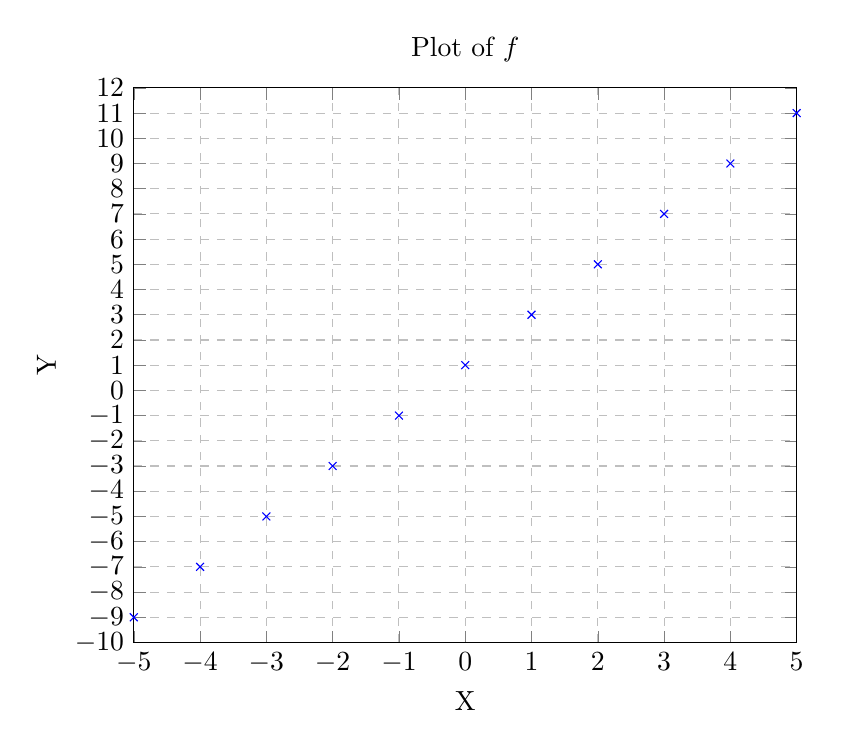
\begin{tikzpicture}
    \begin{axis}[
        title={Plot of $f$},
        xlabel={X},
        ylabel={Y},
        xmin=-5, xmax=5,
        ymin=-10, ymax=12,
        xtick={-5,-4,-3,-2,-1,0,1,2,3,4,5},
        ytick={-10,-9,-8,-7,-6,-5,-4,-3,-2,-1,0,1,2,3,4,5,6,7,8,9,10,11,12},
        %legend pos=north west,
        ymajorgrids=true,
        xmajorgrids=true,
        grid style=dashed,
    ]
    
    \addplot[only marks,mark=x,color=blue] coordinates {(-5,-9)(-4,-7)(-3,-5)(-2,-3)(-1,-1)(0,1)(1,3)(2,5)(3,7)(4,9)(5,11)};
    \end{axis}
    \end{tikzpicture}
%\end{comment}



\hrulefill

\newpage
\item[6.2.8.] Let $g:\Z\times\Z\to\Z\times \Z$ be defined by $g(m,n)=(2m,m-n)$.
\begin{enumerate}[(a)]
\item Calculate $g(3,5)$ and $g(-1,4)$.
\begin{center}
    $g(3,5) = (2(3),3-5) = (6,-2)$\\
    $g(-1,4) = (2(-1),-1-4) = (-2,-5)$\\
\end{center}
\item Determine all the preimages of $(0,0)$. That is, find all $(m,n)\in\Z\times\Z$ such that $g(m,n)=(0,0)$.\\
\indent The set of preimages for $m$ all satisfy $2m = 0$ which is equal to $\{0\}$. From this, we can now find the
set of preimages of $n$ which satisfy
\begin{center}
    $m-n = 0$\\
    $m = n$\\
    and $m = 0$\\
    $\therefore n=0$
\end{center}
Thus the set of preimages of $(0,0)$ are $\{(0,0)\}$.
\item Determine the set of all preimages of $(8,-3)$.\\
\indent The set of preimages for $m$ in this case is $2m = 8\rightarrow m = 4$. From this, we can now find the set
of all preimages of $n$:
\begin{center}
    $g(n) = m-n$\\
    $g(n) - m = -n$\\
    $m-g(n) = n$\\
    from earlier, $m = 4$ and $g(n) = -3$\\
    $\therefore n = 4 - (-3) = 7$
\end{center}
Thus the set of preimages of $(8,-3)$ are $\{(4,7)\}$.

\item Determine the set of all preimages of $(1,1)$.\\
\indent There are no perimages in for $(1,1)$ because $g(m,n)$ is not a surjection of $\Z$\\
In order to get a preimage of $(1,1)$, we need to expand the domain to $\R$ as $2m=1\rightarrow m = \frac{1}{2}$
and $\frac{1}{2} \notin \Z$
\item Is the following proposition true or false? Justify your conclusion.
\begin{quote}
For each $(s,t)\in\Z\times\Z$, there exists $(m,n)\in\Z\times\Z$ such that $g(m,n)=(s,t)$.\\
\indent False. Consider part d of this question. 
\end{quote}

\end{enumerate}

\hrulefill


\item[6.3.8.] 
\begin{enumerate}[(a)]
\item Let $f:\Z\times \Z\to\Z$ be defined by $f(m,n)=2m+n$. Is the function $f$ an injection? Is the function $f$ a surjection? Justify your conclusions.\\
The function $f$ is not an injection as $f(1,1) = f(2,-1) = 3$\\
However, the function $f$ is a surjection:
\begin{center}
    Case 1: y is even $\rightarrow m = \frac{y}{2}\rightarrow f(\frac{y}{2},0) = 2(\frac{y}{2})+0 = y$\\
    Case 2: y is odd $\rightarrow m = \frac{y-1}{2}\rightarrow f(\frac{y-1}{2},1) = 2(\frac{y-1}{2})+1 = y$
\end{center}
Thus the function $f$ is a surjection.
\item Let $g:\Z\times \Z \to\Z$ be defined by $g(m,n)=6m+3n$. Is the function $g$ an injection? Is the function $g$ a surjection? Justify your conclusions.\\
\indent The function $g$ is not an injection as $g(1,1) = 6(1)+3(1) = g(2,-1) = 6(2)+3(-1) = 9$\\
The function $g$ is not a surjection as $g(m,n) = 3(2m+n)$ which means that g(m,n) must be divisible by 3.
Consider $2$ which is an integer and thus in the codomain of $g$ (i.e. $\Z$), yet not divisible by $3$ into an integer $(\frac{2}{3} \approx 0.6667)$
\end{enumerate}
\end{itemize}
\end{document}